\documentclass[border=10pt]{standalone}
\usepackage[dvipsnames]{xcolor}
\usepackage{tikz}
\usetikzlibrary{arrows.meta,positioning,fit,backgrounds,calc}
\usepackage{amsmath}

\definecolor{useC}{RGB}{197,224,180}   % covered/used class
\definecolor{instC}{RGB}{255,224,178}  % instance
\definecolor{w1}{RGB}{142,196,238}
\definecolor{w2}{RGB}{178,214,243}
\definecolor{w3}{RGB}{210,231,248}
\definecolor{w4}{RGB}{233,243,252}

\begin{document}
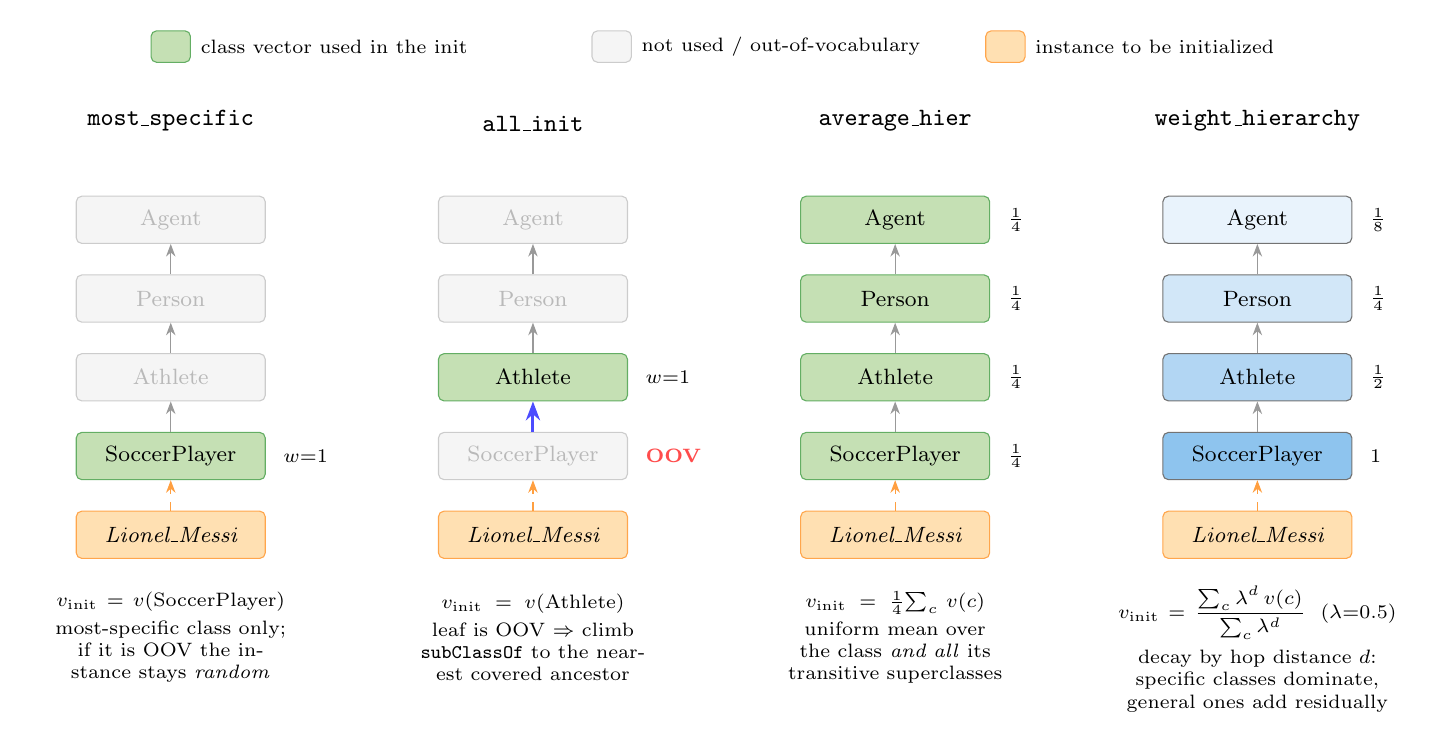
\begin{tikzpicture}[
  font=\footnotesize,
  cls/.style={draw=black!55, rounded corners=2pt, minimum height=6mm,
              minimum width=24mm, inner sep=2pt, fill=white},
  used/.style={cls, fill=useC, draw=ForestGreen!70},
  off/.style={cls, fill=gray!8, draw=gray!40, text=gray!55},
  inst/.style={cls, fill=instC, draw=orange!70, font=\footnotesize\itshape},
  sub/.style={-{Stealth[length=1.6mm]}, draw=black!40},
  typ/.style={-{Stealth[length=1.6mm]}, draw=orange!75, dashed},
  climb/.style={-{Stealth[length=2.4mm]}, draw=blue!70, line width=1.1pt},
  wlab/.style={font=\scriptsize, anchor=west},
  ttl/.style={font=\small\bfseries\ttfamily, anchor=south},
  note/.style={font=\scriptsize, align=center, text width=34mm},
]

% ============ helper coordinates ============
% panel x centres
\def\px{0}     % most_specific
\def\pia{4.6}  % all_init
\def\pib{9.2}  % average_hier
\def\pic{13.8} % weight_hierarchy
% row y for each class box
\def\yA{4.0}\def\yP{3.0}\def\yT{2.0}\def\yS{1.0}\def\yI{0.0}

% ---------------- shared vertical chain drawer via explicit nodes ----------------

% ===================== Panel 1: most_specific =====================
\node[ttl] at (\px,5.0) {most\_specific};
\node[off]  (a1) at (\px,\yA) {Agent};
\node[off]  (p1) at (\px,\yP) {Person};
\node[off]  (t1) at (\px,\yT) {Athlete};
\node[used] (s1) at (\px,\yS) {SoccerPlayer};
\node[inst] (i1) at (\px,\yI) {Lionel\_Messi};
\draw[sub] (s1) -- (t1); \draw[sub] (t1) -- (p1); \draw[sub] (p1) -- (a1);
\draw[typ] (i1) -- (s1);
\node[wlab] at ($(s1.east)+(0.1,0)$) {$w{=}1$};
\node[note] at (\px,-1.3) {$v_{\mathrm{init}}=v(\text{SoccerPlayer})$\\[2pt]
  most-specific class only; if it is OOV the instance stays \emph{random}};

% ===================== Panel 2: all_init =====================
\node[ttl] at (\pia,5.0) {all\_init};
\node[off]  (a2) at (\pia,\yA) {Agent};
\node[off]  (p2) at (\pia,\yP) {Person};
\node[used] (t2) at (\pia,\yT) {Athlete};
\node[off]  (s2) at (\pia,\yS) {SoccerPlayer};
\node[inst] (i2) at (\pia,\yI) {Lionel\_Messi};
\node[font=\scriptsize\bfseries, text=red!70, anchor=west] at ($(s2.east)+(0.1,0)$) {OOV};
\draw[sub] (p2) -- (a2); \draw[sub] (t2) -- (p2);
\draw[climb] (s2) -- (t2);
\draw[typ] (i2) -- (s2);
\node[wlab] at ($(t2.east)+(0.1,0)$) {$w{=}1$};
\node[note] at (\pia,-1.3) {$v_{\mathrm{init}}=v(\text{Athlete})$\\[2pt]
  leaf is OOV $\Rightarrow$ climb \texttt{subClassOf} to the nearest covered ancestor};

% ===================== Panel 3: average_hier =====================
\node[ttl] at (\pib,5.0) {average\_hier};
\node[used] (a3) at (\pib,\yA) {Agent};
\node[used] (p3) at (\pib,\yP) {Person};
\node[used] (t3) at (\pib,\yT) {Athlete};
\node[used] (s3) at (\pib,\yS) {SoccerPlayer};
\node[inst] (i3) at (\pib,\yI) {Lionel\_Messi};
\draw[sub] (s3) -- (t3); \draw[sub] (t3) -- (p3); \draw[sub] (p3) -- (a3);
\draw[typ] (i3) -- (s3);
\foreach \n in {a3,p3,t3,s3}{\node[wlab] at ($(\n.east)+(0.1,0)$) {$\tfrac14$};}
\node[note] at (\pib,-1.3) {$v_{\mathrm{init}}=\tfrac14\!\sum_{c}\, v(c)$\\[2pt]
  uniform mean over the class \emph{and all} its transitive superclasses};

% ===================== Panel 4: weight_hierarchy =====================
\node[ttl] at (\pic,5.0) {weight\_hierarchy};
\node[cls,fill=w4] (a4) at (\pic,\yA) {Agent};
\node[cls,fill=w3] (p4) at (\pic,\yP) {Person};
\node[cls,fill=w2] (t4) at (\pic,\yT) {Athlete};
\node[cls,fill=w1] (s4) at (\pic,\yS) {SoccerPlayer};
\node[inst] (i4) at (\pic,\yI) {Lionel\_Messi};
\draw[sub] (s4) -- (t4); \draw[sub] (t4) -- (p4); \draw[sub] (p4) -- (a4);
\draw[typ] (i4) -- (s4);
\node[wlab] at ($(s4.east)+(0.1,0)$) {$1$};
\node[wlab] at ($(t4.east)+(0.1,0)$) {$\tfrac12$};
\node[wlab] at ($(p4.east)+(0.1,0)$) {$\tfrac14$};
\node[wlab] at ($(a4.east)+(0.1,0)$) {$\tfrac18$};
\node[note, text width=40mm] at (\pic,-1.45) {$v_{\mathrm{init}}=\dfrac{\sum_c \lambda^{d}\,v(c)}{\sum_c \lambda^{d}}$\ \ ($\lambda{=}0.5$)\\[3pt]
  decay by hop distance $d$: specific classes dominate, general ones add residually};

% ============ legend ============
\node[used, minimum width=5mm, minimum height=4mm] (lg1) at (0.0,6.2) {};
\node[anchor=west, font=\scriptsize] at (lg1.east) {class vector used in the init};
\node[off, minimum width=5mm, minimum height=4mm] (lg2) at (5.6,6.2) {};
\node[anchor=west, font=\scriptsize] at (lg2.east) {not used / out-of-vocabulary};
\node[inst, minimum width=5mm, minimum height=4mm] (lg3) at (10.6,6.2) {};
\node[anchor=west, font=\scriptsize] at (lg3.east) {instance to be initialized};

\end{tikzpicture}
\end{document}
